\documentclass[a4paper, czech]{article}

\usepackage[czech]{babel}
\usepackage{indentfirst}
\usepackage{graphicx}
\usepackage{float}
\usepackage[margin=1.5cm]{geometry}
\usepackage{booktabs}
\usepackage{amsmath}
\usepackage{xcolor}
\usepackage{multirow}
\usepackage{tabularray}
\usepackage{bold-extra}
\usepackage{circuitikz}
\usepackage{latexsym}

\begin{document}
\begin{table}[H]
    \centering
    \begin{tblr}{
        cell{1}{1} = {c = 2, r = 4}{c}, % Logo
        cell{1}{4} = {c = 3}{c}, % Předmět
        cell{2}{4} = {c = 3}{c}, % Jméno
        cell{3}{4} = {}{c}, % Ročník
        cell{3}{6} = {}{c}, % Studijní skupina
        cell{4}{4} = {}{c}, % Spolupracoval
        cell{4}{6} = {}{c}, % Mereno dne
        cell{5}{1} = {c = 2}{55mm}, % Kontroloval
        cell{5}{3} = {c = 2}{55mm}, % Hodnoceni
        cell{5}{5} = {c = 2}{55mm}, % Dne
        cell{6}{2} = {c = 5}{}, % Nazev ulohy
        cell{7}{1} = {}{c}, % Číslo úlohy
        cell{7}{2} = {c = 5}{c}, % Název úlohy
        vline{1,2,7} = {1.2pt},
        vline{3,5},
        hline{1,5,6,8} = {1.2pt},
        hline{2,3,4}
        }
        
\includegraphics{logo_fekt.png} & & \textsuperscript{Předmět} & \large \textbf{Měření v audiotechnice} \\
             & & \textsuperscript{Jméno} & \large \textbf{Karolína Šebestová} \\
             & & \textsuperscript{Ročník} & \large \textbf{3.} & \textsuperscript{Studijní skupina} & \large \textbf{St 14:00} \\
             & & \textsuperscript{Spolupracoval} & \large \textbf{Filip Kokavec} & \textsuperscript{Měřeno dne} & \large \textbf{6.11.2024} \\
        \textsuperscript{Kontroloval} & & \textsuperscript{Hodnocení} & & \textsuperscript{Dne} \\
        \textsuperscript{Číslo úlohy} & \textsuperscript{Název úlohy} \\
        \Large \textbf{6A} & \Large \textsc{\textbf{Princip vzorkování a Č/A převodníku}} \\
    \end{tblr}
\end{table}

\section{Zadání}

\begin{itemize}
    \item Experimentálně ověřte funkci vzorkovacího zesilovače:
    \begin{itemize}
        \item znázorněte na osciloskopu průběh výstupního napětí vzorkovače při vzorkování harmonického napětí,
        \item ověřte možnost určení efektivní hodnoty napětí z navzorkovaných hodnot,
        \item v režimu ruční vzorkování sledujte na číslicovém voltmetru změnu hodnoty výstupního napětí v závislosti na čase (chyba pamatování),
        \item na osciloskopu pozorujte průběh napětí na výstupu vzorkovače během tzv. doby upnutí.
    \end{itemize}
    \item U předloženého 8bitového Č/A převodníku experimentálně proměřte převodní charakteristiku. Určete chybu nuly, chybu zesílení a maximální chybu linearity.
    \item Graficky znázorněte převodní charakteristiku Č/A převodníku.
\end{itemize}

\section{Teoretický úvod}

Vzorkovače slouží jako analogová paměť vstupních hodnot signálů a jsou používány zejména v neintegrujících A/Č převodnících.
Jejich funkcí je kvantizace (diskretizace v čase) signálu.
Použitím vzorkování lze určit okamžitou hodnotu spojitého signálu v pravidelném intervalu.
Obvodový prvek odpovědný za paměť je kondenzátor.
Obvykle je zapojen se dvěma operačními zesilovači - jeden urychluje nabíjení kondenzátoru a druhý brání jeho vybíjení.
Pro vzorkovač se běžně používá označení S/H (z anglického Sample and Hold).
Č/A převodníkem ozančujeme zařízení, které převádí vstupní číslicovou hodnotu D reprezentovanou číslem N na výstupní spojité napětí.
\begin{equation*}
    U_a = D \cdot U_{ref} = \frac{N}{2^n} \cdot U_{ref}
\end{equation*}

Vstupní slovo pro osmibitový převodník je definováno jako:
\begin{equation*}
    D = b_7 \cdot 2^{-1} + b_6 \cdot 2^{-2} + ... + b_0 \cdot 2^{-8}
\end{equation*}

Hodnotu maximálního napětí pro osmibitový Č/A převodník lze určit pomocí vztahu:
\begin{equation*}
    U_{a_{max}} = U_{ref} \cdot \left(\frac{1}{2} + \frac{1}{4} + \frac{1}{8} + \frac{1}{16} + \frac{1}{32} + \frac{1}{64} + \frac{1}{128} + \frac{1}{256}\right) = U_{ref} \cdot \frac{255}{256}
\end{equation*}

Rozlišovací schopnost Č/A převodníku je typicky rovna 1 LSB.
Rozlišovací schopnost osmibitového Č/A převodníku je cca. 0,39\,\%.
Nejistota Č/A pŕevodníku je typicky rovna polovině jeho rozlišovací schopnosti, tedy LSB/2.

Převodník DAC08 použitý v této úloze je postaven na bázi integrovaného obvodu WSH 560.
Zdroj referenčního napětí má hodnotu 10,0\,V.
Číslicová vstup pŘevodníku je realizován páčkovými spínači.
Rozsah výstupu lze nastavit přepínačem rozsahu.

Pro správnou funkci vzorkování je potřeba, aby vzorkovací kmitočet byl roven minimálně dvojnásobku hodnoty kmitočtu vzorkovaného spektra.


\begin{figure}[H]
    \centering
    \begin{circuitikz}
        \draw (0,0) to[twoportsplit, t1=$\sim$, t2=$\sqcap\!\sqcup$, l_=Tvarovač] ++(1.5,0)
        node[circ, label=below:$f$](f){} to[twoport, t={\parbox{1cm}{\centering PLL $16 \cdot f$}}, l_=Oscilátor] ++(1.5,0)
        node[circ, label=below:\tiny16\normalsize $f$](16f){} to[twoport, l_=Čítač, t={\parbox{1cm}{\centering výběr 1-16}}] ++(1.5,0)
        node[ocirc, scale=1.5]{} ++(0,0.3) node[ocirc, scale=1.5](A){};
        \draw [line width=2] (A) to ++(0.3,0) coordinate(B);
        \draw (B) ++(0,-0.3) node[ocirc, scale=1.5]{} ++(0,-0.3) node[ocirc, scale=1.5](C){} to ++(0.3,0) ++(-0.6,0) node[ocirc, scale=1.5](D){};
        \draw (A) to ++(0,0.5) coordinate(X) to (X -| 16f) to (16f);
        \draw (B) node[ocirc, scale=1.5]{} to ++(0.3,0) to ++(0,-0.6) node[circ]{} to ++(0,-2.5) to ++(-2.85,0) to ++(0,0.7);
        \draw (0,-2) coordinate(SHin) node[circ]{} to[amp, t=S/H, fill=white, name=vzAMP] ++(4.5,0) coordinate(SHout);
        \draw (SHin) to (0,0);
        \draw [line width=1.2] (-0.75,0) node[ocirc, scale=2](GEN_IN){} to (GEN_IN |- SHin) node[ocirc, scale=1.5](Ux+){} to ++(0,-1.5) node[ocirc, scale=1.5](Ux-){}
        to ++(0,-0.5) to ++(7,0) coordinate(X) to (X |- Ux-) node[ocirc, scale=1.5](Uv-){} to (X |- Ux+) node[ocirc, scale=1.5](Uv+){}
        to ++(0,0.5) node[ocirc, scale=1.5](UvOSC){} to ++(0,0.5) node[ocirc, scale=1.5](Us){} to ++(0,0.5) node[ocirc, scale=1.5](SYN){}
        to ++(0,1.8) coordinate(X) to (X -| GEN_IN) to (GEN_IN);
        \draw (X -| GEN_IN) ++(1,-0.3) node[]{Přípravek};
        \draw (D) to[push button, l_=Ruč. vz.] ++(0,-2) coordinate(X) to (X |- Ux-) node[circ]{};
        \draw (Ux-) to (Uv-);
        \draw (Ux+) to (SHin);
        \draw (Ux-) ++(0.4,0) node[circ]{} to ++(0,3.15) to (GEN_IN);
        \draw (SHout) to (Uv+);
        \draw (SYN) to ++(-0.6,0) to ++(0,1.5) coordinate(X) to (X -| f) to (f);

        \draw (8,0) node[ocirc, scale=1.5, label=\scriptsize Gen](GENout){} ++(1,0) node[ocirc, scale=1.5, label=\tiny CH1](CH1){} ++(0.5,0) node[ocirc, scale=1.5, label=\tiny CH2](CH2){} ++(0.5,0) node[ocirc, scale=1.5, label=\tiny CH3](CH3){} ++(0.5,0) node[ocirc, scale=1.5, label=\tiny CH4](CH4){};
        \draw [line width=1.2] (GENout) ++(-0.3,-0.2) to ++(3.1,0) to ++(0,1.85) to ++(-3.1,0) to ++(0,-1.85);
        \draw (GENout) ++(-0.15,0.5) to ++(1.5,0) to ++(0,1) to ++(-1.5,0) to ++(0,-1);
        \draw (CH3) ++(0,1) node[]{OSC};

        \draw (CH2) to (CH2 |- Us) to (Us);
        \draw (CH3) to (CH3 |- UvOSC) to (UvOSC);
        \draw (GENout) to ++(0,-0.5) node[circ]{};
        \draw (CH1) to ++(0,-0.5) to ++(-2,0) to ++(0,2.2) to ++(-8.5,0) coordinate(X) to (X |- GEN_IN) to (GEN_IN);
        \draw (GEN_IN) ++(-0.4,0.3) node[]{Gen};

        \draw (Uv+) to ++(1,0) to[rmeter, t={V=}] ++(0,-1.5) to (Uv-);
        \draw (Ux+) to ++(-1,0) to[rmeter, t={V$\sim$}] ++(0,-1.5) to (Ux-);

        \draw (SYN) ++(0.3,0.2) node[]{\tiny SYN};
        \draw (Us) ++(0.3,0.2) node[]{\small u$_s$};
        \draw (UvOSC) ++(0.3,0.2) node[]{\small u$_v$};
        \draw (Uv+) ++(0.3,0.2) node[]{\small u$_v$};
        \draw (Ux+) ++(-0.3,0.2) node[]{\small u$_x$};

        \draw (Us) to ++(-1.15,0) node[circ]{};
        \draw (UvOSC) to ++(-0.6,0) to ++(0,-0.5) node[circ]{};

        \draw[-{Straight Barb[angle'=60, scale=2]}] (Ux+) ++(-0.3,-0.2) to ++(0,-1);
        \draw[-{Straight Barb[angle'=60, scale=2]}] (Uv+) ++(0.3,-0.2) to ++(0,-1);
    \end{circuitikz}
    \caption{Zapojení pro ověření funkce vzorkovače napětí}
\end{figure}

\begin{figure}[H]
    \centering
    \begin{circuitikz}
        \draw[-{Straight Barb[angle'=60, scale=2]}] (0,0) to ++(2.5,0);
        \draw (1.25,0.25) node[]{Vstupní slovo};

        \draw [{|[scale=2, line width=1]}-] (2.5,0.5) to ++(0.5,0) coordinate(A);
        \draw [{|[scale=2, line width=1]}-] (2.5,-0.5) to ++(0.5,0) coordinate(B);

        \begin{scope}
            \ctikzset{bipoles/cuteswitch/thickness=0.25}

            \draw (A) to[cute open switch, name=S1, l=$2^7$] ++(1,0) to ++(0.5,0) coordinate(A);
            \draw (B) to[cute open switch, name=S2, l_=$2^0$] ++(1,0) to ++(0.5,0) coordinate(B);
            \draw [densely dashed] (S1.mid) to (S2.mid);
        \end{scope}

        \draw [thick] (A) ++(0,0.5) rectangle ++(2.5,-2) node[pos=0.5, align=center]{8bitový\\D/A\\převodník} coordinate(A);

        \draw (A) ++(0,1) to ++(1,0) coordinate(A);
        \draw [thick] (A) ++(0,0.5) rectangle ++(2,-1) node[pos=0.5]{Voltmetr};
    \end{circuitikz}
    \caption{Blokové schéma pro měření převodníku Č/A}
\end{figure}

\section{Výsledky měření}

\subsection{Tabulky}

\begin{table}[H]
    \catcode`\-=12
    \centering
    \caption{Měření napětí vzorkovačem}
    \begin{tabular}{ll|cccccccc}
        \toprule
        $k$   & [-]  & 0      & 1      & 2      & 3      & 4      & 5      & 6      & 7     \\
        \cmidrule(rl){1-10}
        $U_k$  &  [V]  & -1,210 & -1,950 & -2,380 & -2,450 & -2,160 & -1,530 & -0,660 & 0,288 \\
        $U_k^2$ & [V$^2$] & 1,464  & 3,803  & 5,664  & 6,003  & 4,666  & 2,341  & 0,436  & 0,083 \\
        \midrule
        \midrule
        $k$   & [-]  &8     & 9     & 10    & 11    & 12    & 13    & 14    & 15     \\
        \cmidrule(rl){1-10}
        $U_k$  & [V]  &1,200 & 1,930 & 2,370 & 2,450 & 2,140 & 1,520 & 0,660 & -0,290 \\
        $U_k^2$ & [V$^2$] &1,440 & 3,725 & 5,617 & 6,003 & 4,580 & 2,310 & 0,436 & 0,084 \\
        \bottomrule
        \multicolumn{10}{l}{$U_X = 1,7483$\,V; $U' = 1,744$\,V; $T_A = 1400$\,ns}
    \end{tabular}
\end{table}

\begin{table}[H]
    \catcode`\-=12
    \centering
    \caption{Převodník Č/A}
    \begin{tabular}{ll|ccccccc}
        \toprule
        \multirow{2}{*}{N} & [-]                        & 0      & 16     & 32     & 48     & 64      & 80      & 96      \\
                           & [-]                        & 0      & 10000  & 100000 & 110000 & 1000000 & 1010000 & 1100000 \\
        \cmidrule(rl){1-9}
        $U_{m \check{e} \check{r}}$               & [V] & -5,003 & -4,380 & -3,755 & -3,130 & -2,504  & -1,879  & -1,255  \\
        $U_a$                 & [V]                     & 0,000  & 0,314  & 0,627  & 0,941  & 1,255   & 1,569   & 1,882   \\
        $U_{NP}$                & [V]                   & -5,003 & -4,378 & -3,753 & -3,129 & -2,504  & -1,879  & -1,254  \\
        $\Delta_U$                 & [V]                & 0,000  & -0,002 & -0,002 & -0,001 & 0,000   & 0,000   & -0,001 \\
        \cmidrule(){1-9}
        \morecmidrules
        \cmidrule(){1-9}
        \multirow{2}{*}{N} & [-]                        & 112     & 128      & 144      & 160      & 176      & 192      & 208      \\
         & [-]                        & 1110000 & 10000000 & 10010000 & 10100000 & 10110000 & 11000000 & 11010000 \\
        \cmidrule(rl){1-9}
        $U_{m \check{e} \check{r}}$               & [V] & -0,630  & 0,002    & 0,623    & 1,247    & 1,872    & 2,497    & 3,121    \\
        $U_a$                 & [V]                     & 2,196   & 2,510    & 2,824    & 3,137    & 3,451    & 3,765    & 4,078    \\
        $U_{NP}$                & [V]                   & -0,630  & -0,005   & 0,620    & 1,245    & 1,869    & 2,494    & 3,119    \\
        $\Delta_U$                 & [V]                & 0,000   & 0,007    & 0,003    & 0,002    & 0,003    & 0,003    & 0,002    \\
        \cmidrule(){1-9}
        \morecmidrules
        \cmidrule(){1-5}
        \multirow{2}{*}{N} & [-]                        & 224      & 240      & 255      \\
                   & [-]                        & 11100000 & 11110000 & 11111111 \\
        \cmidrule(rl){1-5}
        $U_{m \check{e} \check{r}}$               & [V] & 3,745    & 4,370    & 4,954    \\
        $U_a$                 & [V]                     & 4,392    & 4,706    & 5,000    \\
        $U_{NP}$                & [V]                   & 3,744    & 4,368    & 4,954    \\
        $\Delta_U$                 & [V]                & 0,001    & 0,002    & 0,000    \\
        \cmidrule[0.8pt]{1-5}
        \multicolumn{9}{l}{$U_{ref} = 5$\,V}
    \end{tabular}
\end{table}

\subsection{Grafy}

\begin{figure}[H]
    \centering
    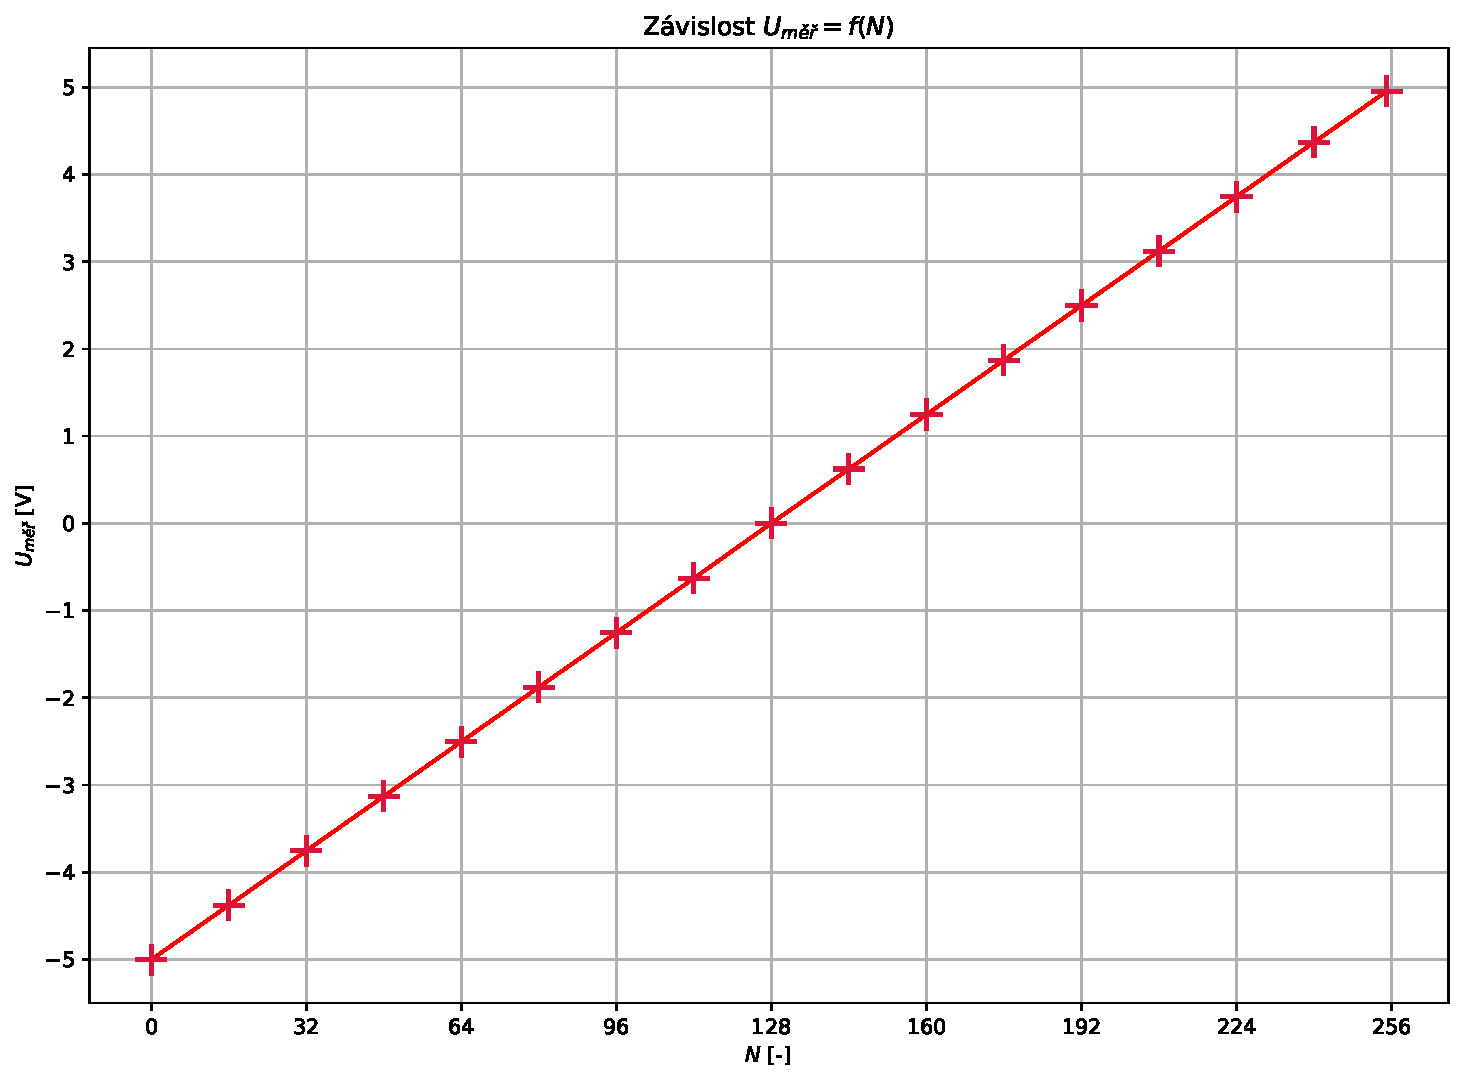
\includegraphics[width=\textwidth]{grafy/graf1.pdf}
    \caption{Převodní charakteristika Č/A převodníku}
\end{figure}

\begin{figure}[H]
    \centering
    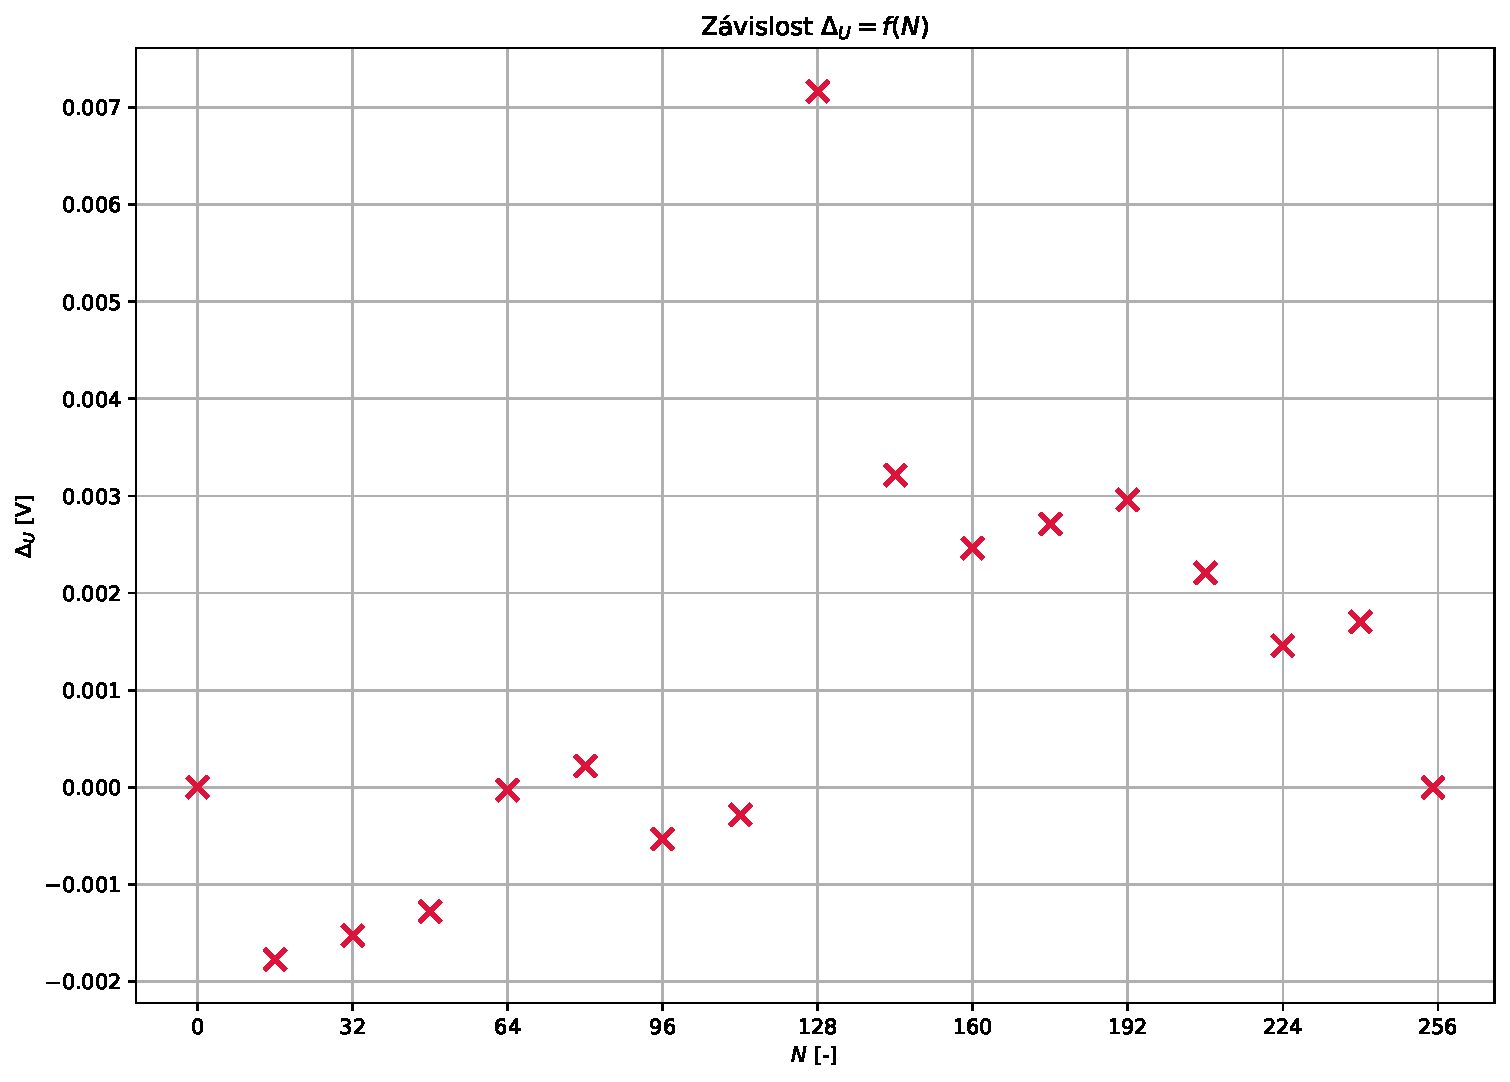
\includegraphics[width=\textwidth]{grafy/graf2.pdf}
    \caption{Průběh chyby v závislosti na vstupním slově} 
\end{figure}

\subsection{Příklady výpočtu}

\begin{enumerate}
    \item Efektivní hodnota vzorkovaného signálu
    \begin{multline*}
        U' = \textcolor{teal}{\sqrt{\frac{1}{N} \sum_{k=0}^{n-1} U_k^2}} = \sqrt{\frac{1}{16} \cdot \left( 1,464 + 3,803 + ... + 0,084 \right)} = \underline{\underline{1,744\,V}} \hfill
    \end{multline*}

    \item Chyba zesílení
    \begin{multline*}
        \Delta_K = \textcolor{teal}{U_{255} - \Delta_{ofs} - U_{ref} \frac{255}{256}} = U_{255} - \Delta_{ofs} - U_{ref} \frac{255}{256} = 4,954\,V - (-5,003\,V) - 5\,V \frac{255}{256} = \underline{\underline{4,976\,V}} \hfill
    \end{multline*}

    \item Napětí odpovídající ideální převodní charakteristice
    \begin{multline*}
        U_a = \textcolor{teal}{U_{ref} \cdot \frac{N}{256}} = 5\,V \cdot \frac{128}{256} = \underline{\underline{2,5\,V}} \hfill
    \end{multline*}

    \item Napětí odpovídající náhradní přímkové charakteristice
    \begin{multline*}
        U_{NP} = \textcolor{teal}{\frac{U_{255} - \Delta_{ofs}}{255} \cdot N + \Delta_{ofs}} = \frac{4,954\,V - (-5,003)}{255} \cdot 128 + (-5,003) = -4,976 \cdot 10^{-3}\,V = \underline{\underline{-4,976\,mV}} \hfill
    \end{multline*}

    \item Odchylka měřeného napětí
    \begin{multline*}
        \Delta_U = \textcolor{teal}{U_{m \check{e} \check{r}} - U_{NP}} = 0,002\,V - (-0,005\,V) = \underline{\underline{0,007\,V}} \hfill
    \end{multline*}

    \item Maximální chyba linearity
    \begin{multline*}
        \Delta_L = \textcolor{teal}{max \left\{\Delta_U\right\}} = \underline{\underline{0,007\,V}} \hfill
    \end{multline*}
\end{enumerate}

\subsection{Snímky obrazovky osciloskopu}

\begin{figure}[H]
    \centering
    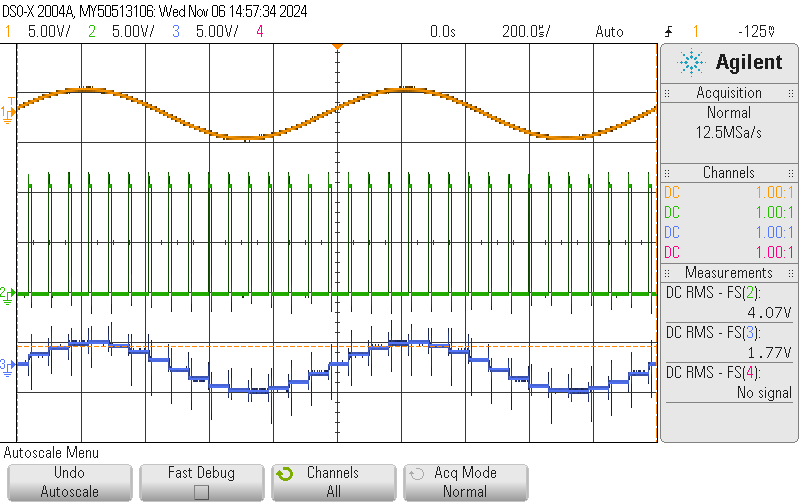
\includegraphics[width=\textwidth]{osc_6A_1.png}
    \caption{Snímek obrazovky osciloskopu}
\end{figure}

\section{Seznam použitých přístrojů}

\begin{itemize}
    \item Laboratorní číslicový multimetr Keysight 34450A, v.č. MY58180038
    \item Číslicový osciloskop Agilent DSO-X 2004A, v.č. MY50513106
\end{itemize}

\section{Závěr}

Úkolem námi provedeného měření bylo experimentálně určit převodní charakteristiku Č/A převodníku a dále určit i jeho chabu nuly, chybu zesílení a také maximální chybu linearity.
Dále bylo potřeba získanou převodní charakteristiku také graficky znázornit.

Námi vypočtená efektivní hodnota napětí zrekonstruovaného signálu $U' = 1,744\,$V je téměř totožná s efektivní hodnotou napětí původního signálu $U_X = 1,7483\,$V.
Také námi určená maximální chyba linearity $\Delta_L = 0,007\,$V při hodnotě $N = 128$ je velice malá.
Chyba v nule je však poměrně velká.
To je způsobeno tím, že naměřená charakteristika je stejnosměrně posunuta do záporných hodnot.

\end{document}